% Choose one to switch between slides and handout
%\documentclass[]{beamer}
\documentclass[handout]{beamer}

% Video Meta Data
\title{Bitcoin, Blockchain and Cryptoassets}
\subtitle{Incentives and Potential Consensus Attacks}
\author{Prof. Dr. Fabian Schär}
\institute{University of Basel}

% Config File
% Packages
\usepackage[utf8]{inputenc}
\usepackage{hyperref}
\usepackage{gitinfo2}
\usepackage{tikz}
\usepackage{amsmath}
\usepackage{mathtools}
\usepackage{bibentry}
\usepackage{xcolor}
\usepackage{colortbl} % Add colour to LaTeX tables
\usepackage{caption}
\usepackage[export]{adjustbox}
\usepackage{pgfplots} \pgfplotsset{compat = 1.17}
\usepackage{makecell}
\usepackage{fancybox}
\usepackage{ragged2e}
\usepackage{fontawesome}
\usepackage{seqsplit}
\usepackage{tabularx}

% Color Options
\definecolor{highlight}{rgb}{0.65,0.84,0.82}
\definecolor{focus}{rgb}{0.72, 0, 0}
\definecolor{lightred}{rgb}{0.8,0.5,0.5}
\definecolor{midgray}{RGB}{190,195,200}

% Beamer Template Options
\beamertemplatenavigationsymbolsempty
\setbeamertemplate{footline}[frame number]
\setbeamercolor{structure}{fg=black}
\setbeamercolor{footline}{fg=black}
\setbeamercolor{title}{fg=black}
\setbeamercolor{frametitle}{fg=black}
\setbeamercolor{item}{fg=black}
\setbeamercolor{}{fg=black}
\setbeamercolor{bibliography item}{fg=black}
\setbeamercolor*{bibliography entry title}{fg=black}
\setbeamercolor{alerted text}{fg=focus}
\setbeamertemplate{items}[square]
\setbeamertemplate{enumerate items}[default]
\captionsetup[figure]{labelfont={color=black},font={color=black}}
\captionsetup[table]{labelfont={color=black},font={color=black}}

\setbeamertemplate{bibliography item}{\insertbiblabel}

% Link Icon Command
\newcommand{\link}{%
    \tikz[x=1.2ex, y=1.2ex, baseline=-0.05ex]{%
        \begin{scope}[x=1ex, y=1ex]
            \clip (-0.1,-0.1)
                --++ (-0, 1.2)
                --++ (0.6, 0)
                --++ (0, -0.6)
                --++ (0.6, 0)
                --++ (0, -1);
            \path[draw,
                line width = 0.5,
                rounded corners=0.5]
                (0,0) rectangle (1,1);
        \end{scope}
        \path[draw, line width = 0.5] (0.5, 0.5)
            -- (1, 1);
        \path[draw, line width = 0.5] (0.6, 1)
            -- (1, 1) -- (1, 0.6);
        }
    }

% Read Git Data from Github Actions Workflow
% Defaults to gitinfo2 for local builds
\IfFileExists{gitInfo.txt}
	{\input{gitInfo.txt}}
	{
		\newcommand{\gitRelease}{(Local Release)}
		\newcommand{\gitSHA}{\gitHash}
		\newcommand{\gitDate}{\gitAuthorIsoDate}
	}

% Custom Titlepage
\defbeamertemplate*{title page}{customized}[1][]
{
  \vspace{-0cm}\hfill\includegraphics[width=2.5cm]{../config/logo_cif}
  \includegraphics[width=1.9cm]{../config/seal_wwz}
  \\ \vspace{2em}
  \usebeamerfont{title}\textbf{\inserttitle}\par
  \usebeamerfont{title}\usebeamercolor[fg]{title}\insertsubtitle\par  \vspace{1.5em}
  \small\usebeamerfont{author}\insertauthor\par
  \usebeamerfont{author}\insertinstitute\par \vspace{2em}
  \usebeamercolor[fg]{titlegraphic}\inserttitlegraphic
    \tiny \noindent \texttt{Release Ver.: \gitRelease}\\ 
    \texttt{Version Hash: \gitSHA}\\
    \texttt{Version Date: \gitDate}\\ \vspace{1em}
    
    
    \iffalse
  \link \href{https://github.com/cifunibas/Bitcoin-Blockchain-Cryptoassets/blob/main/slides/intro.pdf}
  {Get most recent version}\\
  \link \href{https://github.com/cifunibas/Bitcoin-Blockchain-Cryptoassets/blob/main/slides/intro.pdf}
  {Watch video lecture}\\ 
  
  \fi
  
  \vspace{1em}
  License: \texttt{Creative Commons Attribution-NonCommercial-ShareAlike 4.0 International}\\\vspace{2em}
  \includegraphics[width = 1.2cm]{../config/license}
}


% tikzlibraries
\usetikzlibrary{decorations.pathreplacing}
\usetikzlibrary{decorations.markings}
\usetikzlibrary{positioning}
\usetikzlibrary{calc}
\captionsetup{font=footnotesize}


%%%%%%%%%%%%%%%%%%%%%%%%%%%%%%%%%%%%%%%%%%%%%%
%%%%%%%%%%%%%%%%%%%%%%%%%%%%%%%%%%%%%%%%%%%%%%
\begin{document}

\thispagestyle{empty}
\begin{frame}[noframenumbering]
	\titlepage
\end{frame}

%%%
\begin{frame}{Introduction}

By now, we know about the fundamental role of consensus and the dangers of difficulties:
	\begin{itemize}
		\item Danger of permanent network splits.
		\item Uncertainty in case of temporary forks.
	\end{itemize}
	
\vspace{0.5 em}
$\Rightarrow$ Both cases impact value of network to the users.

\vspace{1.5 em}
\uncover<2->{
\textbf{Focus of this lecture:}
	\begin{itemize}
		\item General incentives for consensus relevant nodes (CRNs)
		\item Bitcoin specifics and incentives driving consensus.
		\item Consensus attacks in this context.
	\end{itemize}
}

\end{frame}
%%%

%%%
\begin{frame}{Economic Considerations of a CRN}

To get participants to serve as compliant CRN and bear the corresponding cost, a Blockchain network typically offers revenues.

\vspace{1 em}

\footnotesize
\textbf{General CRN P\&L categories}
\begin{table}
	{\renewcommand{\arraystretch}{1.3}%
  \center
  \begin{tabular}[]{p{0.43\textwidth} | p{0.47\textwidth}}
		\textbf{Cost} & \textbf{Revenues}      \\
		\hline
		Computation & Block-based (e.g., Coinbase tx)\\
		\textit{(electricity, hardware, etc.)} & Transaction-based (e.g., fees)\\
		Cost of stake* & Attestation rewards*\\
		Cost of maintaining Authority* & Miner Extracted Value (MEV)
  \end{tabular}}
\end{table}

\scriptsize *not applicable in Bitcoin context

\vspace{1 em}
\normalsize
$\Rightarrow$ With revenues in network currency and cost often in FIAT, CRNs have an incentive to keep network value - and consequently demand - high.
	
\end{frame}
%%%	

%%%
\begin{frame}{Computing Power Allocation}

\begin{columns}[T]
	\begin{column}{0.45\textwidth}
		\textbf{Mining Market:} \\
		\begin{itemize}
			\item Competitive due to low entry barriers.
			\item Profits only through above average efficiency.
		\end{itemize}		
		
		
		\vspace{1 em}
		\uncover<2->{
			\textbf{Underallocation:} Miners add power to realize more profits.\\}
		
		\vspace{1 em}
		\uncover<3->{
		\textbf{Overallocation:} Miners remove power to avoid losses.}
	\end{column} %\hfill
	\begin{column}{0.55\textwidth}
		\begin{center}
		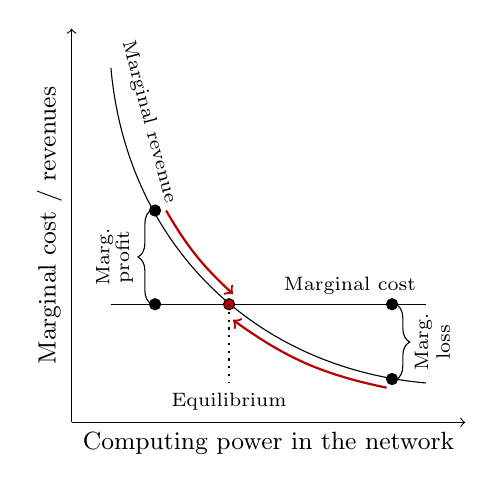
\begin{tikzpicture}[scale=1.0, every node/.style ={scale=1.0}]
			% Title: Equilibrium in Mining Market

% Basics

\uncover<1-3>{
  \draw[->] (0,0)--(5,0) node[below,midway]{\small{Computing power in the network}};
  \draw[->] (0,0)--(0,5) node[above,midway,rotate=90]{\small{Marginal cost / revenues}};
  \draw 	(0.5,1.5) -- (4.5,1.5) node[above left]{\scriptsize{Marginal cost}};
  \draw		(0.45,4.9) node[rotate= -75,above right]{\scriptsize{Marginal revenue}};
  \draw		(4.5,0.5) to[bend left = 40] (0.5,4.5);
  \draw[fill=focus] 	(2,1.5) circle(2pt);
  \draw[dotted,thick] 	(2,1.5) -- (2,0.5) node[below]{\scriptsize{Equilibrium}};

 }
  
% Underallocation

\mode<beamer>{
\uncover<2>{
    \draw[fill=black] (1.06,1.5) circle(2pt);
    \draw[fill=black] (1.06,2.69) circle(2pt);
    \draw [decorate,decoration={mirror, brace,amplitude=5pt},xshift=-8pt,yshift=0pt](1.3,2.7) -- (1.3,1.5) node [black,midway,xshift=-0.6cm, rotate=90] {\scriptsize{Marg.}}node [black,midway,xshift=-0.35cm, rotate=90] {\scriptsize{profit}};
    \draw [color = focus,->,thick] (1.2,2.69) to[bend right = 8.5] (2.05,1.63);

 }


% Overallocation

\uncover<3>{
    \draw[fill=black] (4.07,1.5) circle(2pt);
    \draw[fill=black] (4.07,0.55) circle(2pt);
    \draw [decorate,decoration={brace,amplitude=5pt},xshift=-8pt,yshift=0pt](4.4,1.5) -- (4.4,0.54) node [black,midway,xshift=0.35cm, rotate=90] {\scriptsize{Marg.}}node [black,midway,xshift=0.6cm, rotate=90] {\scriptsize{loss}};
    \draw [color = focus,->,thick] (4.0,0.44) to[bend left = 12] (2.05,1.3);
    
 }

}
		\end{tikzpicture}
		\end{center}
	\end{column}
\end{columns}

	
\end{frame}
%%%	

%%%
\begin{frame}{Bitcoin Mining: Probabilistic Reward Distribution}

Under proof-of-work, probability of mining a block and earning the corresponding reward $P$ is defined by a miner $i$'s computing power relative to the network, i.e., $E(p_{i}) = P  \cdot \frac{c_{i}}{C}$.

%ToDo: Expected value / Pi instead of overline R

\vspace{1.5 em}

\uncover<2->{
\textbf{Illustrative example} with P = 6.25 Bitcoin:

\begin{center}
	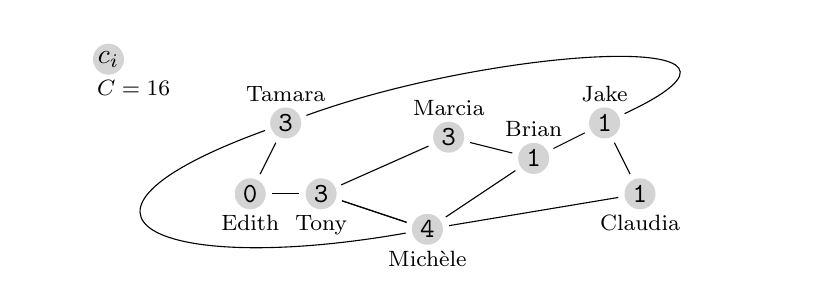
\begin{tikzpicture}[scale=0.9, every node/.style ={scale=1.0}]
		% Illustrative network of CRNs with respective computing power

% Colors

\definecolor{lgrey}{rgb}{0.83,0.83,0.83}


% Outline
\coordinate (c1) at (0,0);
\coordinate (c2) at (1,0);
\coordinate (c3) at (2.8,0.8);
\coordinate (c4) at (2.5,-0.5);
\coordinate (c5) at (4,0.5);
\coordinate (c6) at (5,1);
\coordinate (c7) at (5.5,0);
\coordinate (c8) at (0.5,1);
\coordinate (L1) at (-2,1.9);
\coordinate (L2) at (-2.3,1.5);

% Nodes
\filldraw[color=lgrey] (c1) circle (6pt) node[color=black]{\texttt{0}} node[below=0.15cm,color=black]{\footnotesize{Edith}};
\filldraw[color=lgrey] (c2) circle (6pt) node[color=black]{\texttt{3}} node[below=0.15cm,color=black]{\footnotesize{Tony}};
\filldraw[color=lgrey] (c3) circle (6pt) node[color=black]{\texttt{3}} node[above=0.15cm,color=black]{\footnotesize{Marcia}};
\filldraw[color=lgrey] (c4) circle (6pt) node[color=black]{\texttt{4}} node[below=0.15cm,color=black]{\footnotesize{Michèle}};
\filldraw[color=lgrey] (c5) circle (6pt) node[color=black]{\texttt{1}} node[above=0.15cm,color=black]{\footnotesize{Brian}};
\filldraw[color=lgrey] (c6) circle (6pt) node[color=black]{\texttt{1}} node[above=0.15cm,color=black]{\footnotesize{Jake}};
\filldraw[color=lgrey] (c7) circle (6pt) node[color=black]{\texttt{1}} node[below=0.15cm,color=black]{\footnotesize{Claudia}};
\filldraw[color=lgrey] (c8) circle (6pt) node[color=black]{\texttt{3}} node[above=0.15cm,color=black]{\footnotesize{Tamara}};

% Connections
\draw[shorten >=0.28cm,shorten <=0.28cm] (c1) to[] (c2);
\draw[shorten >=0.28cm,shorten <=0.28cm] (c2) to[] (c3);
\draw[shorten >=0.28cm,shorten <=0.28cm] (c2) to[] (c4);
\draw[shorten >=0.28cm,shorten <=0.28cm] (c2) to[] (c4);
\draw[shorten >=0.28cm,shorten <=0.28cm] (c3) to[] (c5);
\draw[shorten >=0.28cm,shorten <=0.28cm] (c4) to[] (c5);
\draw[shorten >=0.28cm,shorten <=0.28cm] (c4) to[] (c7);
\draw[shorten >=0.28cm,shorten <=0.28cm] (c5) to[] (c6);
\draw[shorten >=0.28cm,shorten <=0.28cm] (c7) to[] (c6);
\draw[shorten >=0.28cm,shorten <=0.28cm] (c8) to[] (c1);

% add overlay as hack to avoid a lot of whitespace around the picture
\uncover<1->{
\draw[shorten >=0.28cm,shorten <=0.28cm] (c8) to[out = 200, in = 190, distance=110] (c4);
\draw[shorten >=0.28cm,shorten <=0.28cm] (c8) to[out = 20, in = 25, distance=90] (c6);
}

% Legend
\filldraw[color=lgrey] (L1) circle (6pt) node[color=black]{\texttt{$c_{i}$}};
\node	at (L2)[right, text = black]{\footnotesize $C = 16$};
	\end{tikzpicture}
\end{center}

Jake's expected payout per block: $6.25 \cdot \frac{1}{16} = 0.391$ Bitcoin.
}
\end{frame}
%%%	

%%%
\begin{frame}{The Case for Mining Pools}

	\begin{enumerate}
		\item Successful mining of a block follows a Poisson distribution.
		\item Short- to mid-term actual payouts may deviate significantly.
		\item Relatively small miners are disproportionally affected.
	\end{enumerate}

\vspace{1 em}

\uncover<2->{
To address this, Jake, Brian and Claudia can form a \textbf{Mining Pool}:

\begin{center}
	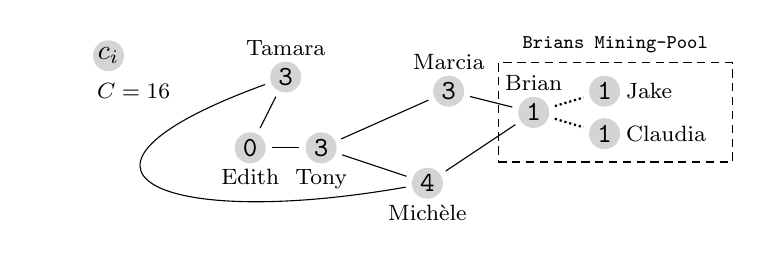
\begin{tikzpicture}[scale=0.9, every node/.style ={scale=1.0}]
		% Illustrative network of CRNs with respective computing power

% Colors

\definecolor{lgrey}{rgb}{0.83,0.83,0.83}


% Outline
\coordinate (c1) at (0,0);
\coordinate (c2) at (1,0);
\coordinate (c3) at (2.8,0.8);
\coordinate (c4) at (2.5,-0.5);
\coordinate (c5) at (4,0.5);
\coordinate (c6) at (5,0.8);
\coordinate (c7) at (5,0.2);
\coordinate (c8) at (0.5,1);
\coordinate (L1) at (-2,1.3);
\coordinate (L2) at (-2.3,0.8);

% Nodes
\filldraw[color=lgrey] (c1) circle (6pt) node[color=black]{\texttt{0}} node[below=0.15cm,color=black]{\footnotesize{Edith}};
\filldraw[color=lgrey] (c2) circle (6pt) node[color=black]{\texttt{3}} node[below=0.15cm,color=black]{\footnotesize{Tony}};
\filldraw[color=lgrey] (c3) circle (6pt) node[color=black]{\texttt{3}} node[above=0.15cm,color=black]{\footnotesize{Marcia}};
\filldraw[color=lgrey] (c4) circle (6pt) node[color=black]{\texttt{4}} node[below=0.15cm,color=black]{\footnotesize{Michèle}};
\filldraw[color=lgrey] (c5) circle (6pt) node[color=black]{\texttt{1}} node[above=0.15cm,color=black]{\footnotesize{Brian}};
\filldraw[color=lgrey] (c6) circle (6pt) node[color=black]{\texttt{1}} node[right=0.15cm,color=black]{\footnotesize{Jake}};
\filldraw[color=lgrey] (c7) circle (6pt) node[color=black]{\texttt{1}} node[right=0.15cm,color=black]{\footnotesize{Claudia}};
\filldraw[color=lgrey] (c8) circle (6pt) node[color=black]{\texttt{3}} node[above=0.15cm,color=black]{\footnotesize{Tamara}};

% Connections
\draw[shorten >=0.28cm,shorten <=0.28cm] (c1) to[] (c2);
\draw[shorten >=0.28cm,shorten <=0.28cm] (c2) to[] (c3);
\draw[shorten >=0.28cm,shorten <=0.28cm] (c2) to[] (c4);
\draw[shorten >=0.28cm,shorten <=0.28cm] (c3) to[] (c5);
\draw[shorten >=0.28cm,shorten <=0.28cm] (c4) to[] (c5);
\draw[shorten >=0.28cm,shorten <=0.28cm, densely dotted,thick] (c5) to[] (c7);
\draw[shorten >=0.28cm,shorten <=0.28cm, densely dotted,thick] (c5) to[] (c6);

\draw[shorten >=0.28cm,shorten <=0.28cm] (c8) to[] (c1);
\draw[shorten >=0.28cm,shorten <=0.28cm] (c8) to[out = 200, in = 190, distance=110] (c4);

%Pool
\draw[densely dashed] (3.5,-0.2)--(6.8,-0.2)--(6.8,1.2)--(3.5,1.2)node[midway,above]{\scriptsize{\texttt{Brians Mining-Pool}}}--(3.5,-0.2);

% Legend
\filldraw[color=lgrey] (L1) circle (6pt) node[color=black]{\texttt{$c_{i}$}};
\node	at (L2)[right, text = black]{\footnotesize $C = 16$};
	\end{tikzpicture}
\end{center}

$ \Rightarrow E(p)$ per block: $6.25 \cdot \frac{1}{16}$ vs. $\frac{6.25}{3} \cdot \frac{3}{16}$.

\vspace{0.5 em}
$\Rightarrow \sigma_{p}$ per block:  $1.523$ vs. \color{focus} \textbf{$0.813$}
}	

\end{frame}
%%%	

%%%
\begin{frame}{Bitcoin Consensus Incentives: Basic Assumptions}

\textbf{CRN operators are:}
\begin{itemize}
	\item	Rational agents\\$\Rightarrow$ Effort is dedicated to chain with highest probability weighted payout.
	\item	Independent (otherwise considered Mining Pools)
\end{itemize}

\vspace{1.5 em}

\uncover<2->{
\textbf{Value of payout is tied to network value}:
\begin{itemize}
	\item	Consensus deviations impair trust in network and thus demand.
	\item	Reduced demand is reflected in lower fees and devaluation of reward currency.
\end{itemize}
}

\end{frame}
%%%	

%%%
\begin{frame}{Bitcoin: Attraction of the Longest Chain}

\textbf{Situation:} Michèle has successfully mined Block 4. Our Mining Pool is considering to continue mining it's own Block 4.

\begin{center}
	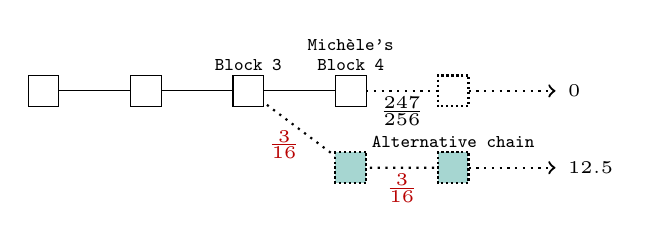
\begin{tikzpicture}[scale=1.3, every node/.style ={scale=1.3}]
		% Title: Scenario of not accepting blocks


% Arrangement
\coordinate	(o0) at	(0,1);
\coordinate (o1) at (1,1);
\coordinate (o2) at (2,1);
\coordinate (o3) at (3,1);
\coordinate (o4) at (4,1);
\coordinate (o45) at (4.5,1);
\coordinate (o5) at (5,1);
\coordinate (o6) at (6,1);
\coordinate (o7) at (7,1);
\coordinate (o8) at (8,1);
\coordinate (o9) at (9,1);
\coordinate (o10) at (10,1);
\coordinate (n1) at (1,0.25);
\coordinate (n2) at (2,0.25);
\coordinate (n3) at (3,0.25);
\coordinate	(on34) at (3.5,0.625);
\coordinate (n4) at (4,0.25);
\coordinate (n45) at (4.5,0.25);
\coordinate (n5) at (5,0.25);
\coordinate (n6) at (6,0.25);
\coordinate (n7) at (7,0.25);
\coordinate (n8) at (8,0.25);
\coordinate (n9) at (9,0.25);
\coordinate (n10) at (10,0.25);

% Chain Lines
\draw[] (o1) -- (o2) -- (o3) -- (o4) ;
\draw[dotted, thick] (o4) -- (o5);
\draw[dotted, thick] (o3) -- (n4) -- (n5);
%\draw[color=black] (n6) to[] (o7);
%\draw[color=black,densely dashed] (o4) to[] (o5);
%\draw[color=black,densely dashed] (o7) to[] (o8);
\draw[color=black,thick, dotted, ->] (o5) to[] (o6);
\draw[color=black,thick, dotted, ->] (n5) to[] (n6);

% Blocks
\node (rect) at (o1) [fill=white,draw,minimum width=0.3cm,minimum height=0.3cm] {};
\node (rect) at (o2) [fill=white,draw,minimum width=0.3cm,minimum height=0.3cm] {};
\node (rect) at (o3) [fill=white,draw,minimum width=0.3cm,minimum height=0.3cm] {};
\node (rect) at (o4) [fill=white,draw,minimum width=0.3cm,minimum height=0.3cm] {};
\node (rect) at (o5) [thick,fill=white,draw,minimum width=0.3cm,minimum height=0.3cm,densely dotted] {};

\node (rect) at (n4) [thick,fill=highlight,draw,minimum width=0.3cm,minimum height=0.3cm,densely dotted] {};
\node (rect) at (n5) [thick,fill=highlight,draw,minimum width=0.3cm,minimum height=0.3cm,densely dotted] {};



% Labels
\node at (o3) [above=0.1cm]{\tiny{\texttt{Block 3}}};
\node at (o4) [above=0.1cm]{\tiny{\texttt{Block 4}}};

\uncover<-1>{
\node at (o4) [above=0.35cm]{\tiny{\texttt{Michèle's}}};
\node at (n5) [above = 0.1cm]{\tiny{\texttt{Alternative chain}}};
}

\uncover<2->{
<2->\node at(on34)[xshift= -0.15cm, yshift=-0.15cm]{\color{focus}\tiny{$\frac{3}{16}$}};
<2->\node at(o45)[yshift=-0.2cm] {\color{black}\tiny{$\frac{247}{256}$}};
<2-> \node at(n45)[yshift=-0.2cm]{\color{focus}\tiny{$\frac{3}{16}$}};
<2-> \node at(n6)[right]{\color{black}\tiny{$12.5$}};
<2-> \node at(o6)[right]{\color{black}\tiny{$0$}};
}
	\end{tikzpicture}
\end{center}

\uncover<2->{
\begin{itemize}
	\item	Consensus compliant CRN's mine on top of Michèle's block.
	\item	To become the longest chain, the Pool must mine two blocks before current consensus chain is extended.
	\item	In case of success, the Pool receives two block rewards.
\end{itemize}

\vspace{0.5 em}
\textbf{Expected Payout:} $\frac{3}{16} \cdot \frac{3}{16} \cdot (6.25 \cdot 2) = 0.439$
}

\end{frame}
%%%	

%%%
\begin{frame}{Bitcoin: Attraction of the Longest Chain (cont.)}

Expected payout over two blocks on top of Michèle's Block 4:

\begin{center}
	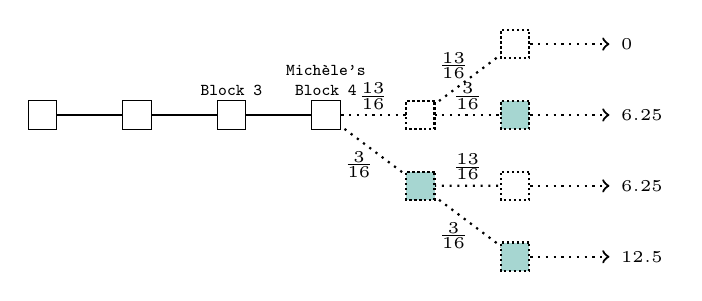
\begin{tikzpicture}[scale=1.2, every node/.style ={scale=1.2}]
		% Title: Scenario of not accepting blocks


% Arrangement

\coordinate (ot45) at (4.5,1.375);
\coordinate (t5) at (5,1.75);
\coordinate (t6) at (6,1.75);

\coordinate	(o0) at	(0,1);
\coordinate (o1) at (1,1);
\coordinate (o2) at (2,1);
\coordinate (o3) at (3,1);
\coordinate (o34) at (3.5,1);
\coordinate (o4) at (4,1);
\coordinate (o45) at (4.5,1);
\coordinate (o5) at (5,1);
\coordinate (o6) at (6,1);


\coordinate	(on34) at (3.5,0.625);
\coordinate (n4) at (4,0.25);
\coordinate (n45) at (4.5,0.25);
\coordinate (n5) at (5,0.25);
\coordinate (n6) at (6,0.25);

\coordinate (nb45) at (4.5,-0.125);
\coordinate (b5) at (5,-0.5);
\coordinate (b6) at (6,-0.5);



% Chain Lines
\draw[] (o0) -- (o1) -- (o2) -- (o3);

\draw[dotted, thick] (o4) -- (t5);
\draw[dotted, thick] (o3) -- (o4) -- (o5);
\draw[dotted, thick] (o3) -- (n4) -- (n5);
\draw[dotted, thick] (n4) -- (b5);

\draw[color=black,thick, dotted, ->] (t5) to[] (t6);
\draw[color=black,thick, dotted, ->] (o5) to[] (o6);
\draw[color=black,thick, dotted, ->] (n5) to[] (n6);
\draw[color=black,thick, dotted, ->] (b5) to[] (b6);


% Blocks
\node (rect) at (o0) [fill=white,draw,minimum width=0.3cm,minimum height=0.3cm] {};
\node (rect) at (o1) [fill=white,draw,minimum width=0.3cm,minimum height=0.3cm] {};
\node (rect) at (o2) [fill=white,draw,minimum width=0.3cm,minimum height=0.3cm] {};
\node (rect) at (o3) [fill=white,draw,minimum width=0.3cm,minimum height=0.3cm] {};

\node (rect) at (o4) [thick,fill=white,draw,minimum width=0.3cm,minimum height=0.3cm,densely dotted]{};
\node (rect) at (t5) [thick,fill=white,draw,minimum width=0.3cm,minimum height=0.3cm,densely dotted] {};
\node (rect) at (n5) [thick,fill=white,draw,minimum width=0.3cm,minimum height=0.3cm,densely dotted]{};

\node (rect) at (o5) [thick,fill=highlight,draw,minimum width=0.3cm,minimum height=0.3cm,densely dotted] {};
\node (rect) at (n4) [thick,fill=highlight,draw,minimum width=0.3cm,minimum height=0.3cm,densely dotted] {};
\node (rect) at (b5) [thick,fill=highlight,draw,minimum width=0.3cm,minimum height=0.3cm,densely dotted] {};



% Labels

\uncover<-1>{
\node at (o2) [above=0.1cm]{\tiny{\texttt{Block 3}}};
\node at (o3) [above=0.1cm]{\tiny{\texttt{Block 4}}};
\node at (o3) [above=0.35cm]{\tiny{\texttt{Michèle's}}};
%\node at (n5) [above = 0.1cm]{\tiny{\texttt{Alternative chain}}};
}

\uncover<2->{
\node at(ot45)[xshift= -0.15cm, yshift=0.15cm]{\color{black}\tiny{$\frac{13}{16}$}};
\node at(o34)[yshift= 0.2cm]{\color{black}\tiny{$\frac{13}{16}$}};
\node at(o45)[yshift=0.2cm] {\color{black}\tiny{$\frac{3}{16}$}};
\node at(on34)[xshift= -0.15cm, yshift=-0.15cm]{\color{black}\tiny{$\frac{3}{16}$}};
\node at(n45)[yshift=0.2cm] {\color{black}\tiny{$\frac{13}{16}$}};
\node at(nb45)[xshift= -0.15cm, yshift=-0.15cm]{\color{black}\tiny{$\frac{3}{16}$}};
}

\node at(t6)[right]{\color{black}\tiny{$0$}};
\node at(o6)[right]{\color{black}\tiny{$6.25$}};
\node at(n6)[right]{\color{black}\tiny{$6.25$}};
\node at(b6)[right]{\color{black}\tiny{$12.5$}};

	\end{tikzpicture}
\end{center}
\uncover<2->{
$\Rightarrow \frac{39}{256} \cdot 6.25 + \frac{39}{256} \cdot 6.25 + \frac{9}{256} \cdot 12.5 = \textbf{2.344}$

\vspace{1 em}
\textbf{Conclusion:}
\begin{itemize}
	\item	Expected payouts strongly support compliance with consensus.
	\item	Relative computing power thresholds for rational deviations are $\ge \frac{2}{3}$ over two blocks and  $\ge \frac{1}{2}$ over long-term.
\end{itemize}
}

\end{frame}
%%%	

%%%
\begin{frame}{Longest Chain Incentives and Process-based Forks}

\textbf{Probabilistic Block Race}
\begin{itemize}
	\item	Expected payout drives fast resolution along "winning" chain. 
	\item	Only miner of abandoned block has skewed incentives.
\end{itemize}

\vspace{0.5 em}

\textbf{Block Withholding / Selfish Mining}
\begin{itemize}
	\item	Risk of loosing block reward $t$ vs. increased chances on $t+1$.
	\item	Only rational for high relative computing power.
\end{itemize}

\vspace{0.5 em}

\textbf{Forced Block Race}
\begin{itemize}
	\item	Longest chain incentives do not discriminate "attack" chains.
	\item	Only rational in case of computing power $\ge 51\%$.
\end{itemize}

\vspace{1.0 em}

$\Rightarrow$ Bitcoin incentives effectively protect consensus in absence of mining power concentration.

\end{frame}
%%%	

%%%
\begin{frame}{Other MEV: Double Spend Attack}

Miners can choose which transactions to include in a block and thus can influence the consensus chain and, for example :
\begin{itemize}
	\item	Deliberately delay a transaction (blocking).
	\item	Attack a block with conflicting transactions (double spend).
\end{itemize}

\vspace{0.5 em}
$\Rightarrow$ Situative other MEV may skew incentives for CRNs.

\uncover<2->{
\vspace{1.0 em}
\textbf{Example:} Raphael pays 10 Bitcoin to Lucas and receives a car. \uncover<3->{Driving away, he attacks Block 4 spending the UTXO on himself.}

\begin{center}
	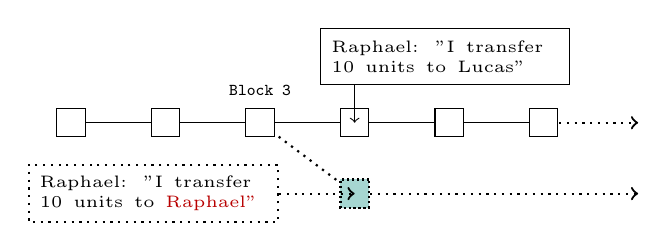
\begin{tikzpicture}[scale=1.2, every node/.style ={scale=1.2}]
		% Title: Miner Double Spend Attack


% Arrangement

\coordinate (o1) at (1,1);
\coordinate (o2) at (2,1);
\coordinate (o3) at (3,1);
\coordinate (o4) at (4,1);
\coordinate (o5) at (5,1);
\coordinate (o6) at (6,1);
\coordinate (o7) at (7,1);

\coordinate (n4) at (4,0.250);
\coordinate (n5) at (5,0.250);
\coordinate (n6) at (6,0.250);
\coordinate (n7) at (7,0.250);

\coordinate (a0) at (4,1.4);
\coordinate (a1) at (3.8,1.7);


\coordinate (b0) at (3.2,0.25);


% Blocks and Connections

\draw[] (o1) -- (o2) -- (o3) -- (o4) -- (o5) --(o6) ;
\draw[color=black,thick, dotted, ->] (o6) to[] (o7);


\uncover<3->{
\draw[thick, dotted] (o3) -- (n4); 
\draw[color=black,thick, dotted, ->] (n4) to[] (n7);
\node (rect) at (n4) [thick, densely dotted,fill=highlight,draw,minimum width=0.3cm, minimum height=0.3cm] {};
}

\node (rect) at (o1) [fill=white,draw,minimum width=0.3cm,minimum height=0.3cm] {};
\node (rect) at (o2) [fill=white,draw,minimum width=0.3cm,minimum height=0.3cm] {};
\node (rect) at (o3) [fill=white,draw,minimum width=0.3cm,minimum height=0.3cm] {};

\node (rect) at (o4) [fill=white,draw,minimum width=0.3cm,minimum height=0.3cm] {};
\node (rect) at (o5) [fill=white,draw,minimum width=0.3cm,minimum height=0.3cm] {};
\node (rect) at (o6) [fill=white,draw,minimum width=0.3cm,minimum height=0.3cm] {};

% Labeling

\node at (o3) [above=0.2cm]{\tiny{\texttt{Block 3}}};

\draw[->] 	(a0) -- (o4);

\linespread{0.5}
\node (rect) at (a1) [draw,right = -0.2cm,text width=2.4cm, minimum height=0.6cm,align = left] {\tiny {Raphael: "I transfer 10 units to Lucas"}};

\uncover<3->{
\draw[->, thick,dotted] 	(b0) -- (n4);
\node (rect) at (b0) [draw,thick, dotted, left,text width=2.4cm, minimum height=0.6cm,align = left] {\tiny {Raphael: "I transfer 10 units to \color{focus} Raphael"}};
}
	\end{tikzpicture}
\end{center}

}

\end{frame}
%%%	

%%%
\begin{frame}{Double Spend Attack without Mining}

\textbf{Scenario}
\begin{itemize}
	\item	Raphael buys take-away coffee, paying in Bitcoin.
	\item	He receives the coffee against the - yet unconfirmed - trx.
	\item<2-> To another node, he sends a trx to himself with the same UTXO.
\end{itemize}

\uncover<3->{
\vspace{0.5 em}
The faster the trxs are propagated through the network, the higher their relative chances to be included in a valid block first:
}

\begin{center}
	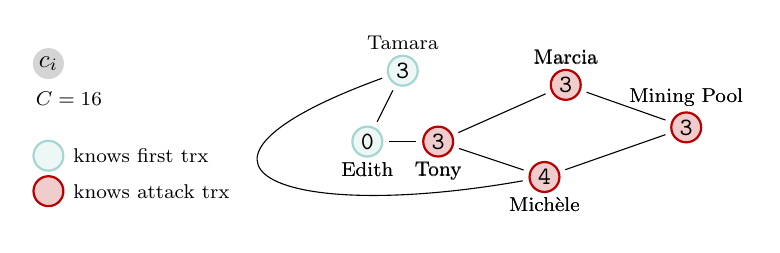
\begin{tikzpicture}[scale=0.9, every node/.style ={scale=0.9}]
		% Double spend attack w/o mining power

% Colors

\definecolor{lgrey}{rgb}{0.83,0.83,0.83}


% Outline
\coordinate (c1) at (0,0);
\coordinate (c2) at (1,0);
\coordinate (c3) at (2.8,0.8);
\coordinate (c4) at (2.5,-0.5);
\coordinate (c5) at (4.5,0.2);
\coordinate (c6) at (5,0.8);
\coordinate (c7) at (5,0.2);
\coordinate (c8) at (0.5,1);

\coordinate (L1) at (-4.5,1.1);
\coordinate (L2) at (-4.8,0.6);
\coordinate (L3) at (-4.5,-0.2);
\coordinate (L4) at (-4.5,-0.7);

% Nodes
\uncover<-2>{
\filldraw[color=lgrey] (c1) circle (6pt) node[color=black]{\texttt{0}} node[below=0.15cm,color=black]{\footnotesize{Edith}};
}
\uncover<3->{
\filldraw[color=highlight, fill = highlight!20, thick] (c1) circle (6pt) node[color=black]{\texttt{0}} node[below=0.15cm,color=black]{\footnotesize{Edith}};
}

\uncover<-2>{
\filldraw[color=lgrey] (c2) circle (6pt) node[color=black]{\texttt{3}} node[below=0.15cm,color=black]{\footnotesize{Tony}};
}
\uncover<3->{
\filldraw[color=focus, fill = focus!20, thick] (c2) circle (6pt) node[color=black]{\texttt{3}} node[below=0.15cm,color=black]{\footnotesize{Tony}};
}

\uncover<-3>{
\filldraw[color=lgrey] (c3) circle (6pt) node[color=black]{\texttt{3}} node[above=0.15cm,color=black]{\footnotesize{Marcia}};
}
\uncover<4->{	
	\filldraw[color=focus, fill = focus!20, thick] (c3) circle (6pt) node[color=black]{\texttt{3}} node[above=0.15cm,color=black]{\footnotesize{Marcia}};
}

\uncover<-1>{
\filldraw[color=lgrey] (c4) circle (6pt) node[color=black]{\texttt{4}} node[below=0.15cm,color=black]{\footnotesize{Michèle}};
}
\uncover<2->{	
	\filldraw[color=focus, fill = focus!20, thick] (c4) circle (6pt) node[color=black]{\texttt{4}} node[below=0.15cm,color=black]{\footnotesize{Michèle}};
}

\uncover<-2>{
\filldraw[color=lgrey] (c5) circle (6pt) node[color=black]{\texttt{3}} node[above=0.15cm,color=black]{\footnotesize{Mining Pool}};
}
\uncover<3->{
\filldraw[color=focus, fill = focus!20, thick] (c5) circle (6pt) node[color=black]{\texttt{3}} node[above=0.15cm,color=black]{\footnotesize{Mining Pool}};
}

\filldraw[color=highlight, fill = highlight!20, thick] (c8) circle (6pt) node[color=black]{\texttt{3}} node[above=0.15cm,color=black]{\footnotesize{Tamara}};

% Connections
\draw[shorten >=0.28cm,shorten <=0.28cm] (c1) to[] (c2);
\draw[shorten >=0.28cm,shorten <=0.28cm] (c2) to[] (c3);
\draw[shorten >=0.28cm,shorten <=0.28cm] (c2) to[] (c4);
\draw[shorten >=0.28cm,shorten <=0.28cm] (c3) to[] (c5);
\draw[shorten >=0.28cm,shorten <=0.28cm] (c4) to[] (c5);
\draw[shorten >=0.28cm,shorten <=0.28cm] (c8) to[] (c1);
\draw[shorten >=0.28cm,shorten <=0.28cm] (c8) to[out = 200, in = 190, distance=110] (c4);


% Legend
\filldraw[color=lgrey] (L1) circle (6pt) node[color=black]{\texttt{$c_{i}$}};
\node	at (L2)[right, text = black]{\footnotesize $C = 16$};

\filldraw[color=highlight, fill = highlight!20, thick] (L3) circle (6pt) node[right = 0.2cm, color=black]{\footnotesize{knows first trx}};

\uncover<2->{
\filldraw[color=focus, fill = focus!20, thick] (L4) circle (6pt) node[right = 0.2cm, color=black]{\footnotesize{knows attack trx}};
}

	\end{tikzpicture}
\end{center}

\uncover<4->{
$\Rightarrow$ Relayed to a better connected node, the attack trx is probably getting confirmed first, leaving Raphael with coffee AND Bitcoin.}

\end{frame}
%%%	

%%%
\begin{frame}{Double Spend Attack without Mining (cont.)}

Double spend attacks \color{focus} do not require own mining power.\color{black} The chances of success are not negligible, given enough time pressure in the exchange payment vs. goods.
\vspace{1.5 em}

\uncover<2->{
The payee can take \textbf{cautionary measures} to minimize success probability of such attacks:

\vspace{0.5 em}
\begin{itemize}
	\item	If not waiting for confirmation, at least a minimal waiting time between relaying transaction and handing out goods.
	\item	Maintaining a broad network connection to foster propagation of own transaction and increase chances of becoming aware of conflicting transactions.
\end{itemize}
}


\end{frame}
%%%	


%%%
\begin{frame}%[allowframebreaks]
\frametitle{References and Recommended Reading}

		\begin{columns}[T]
			\begin{column}{0.1\textwidth}
					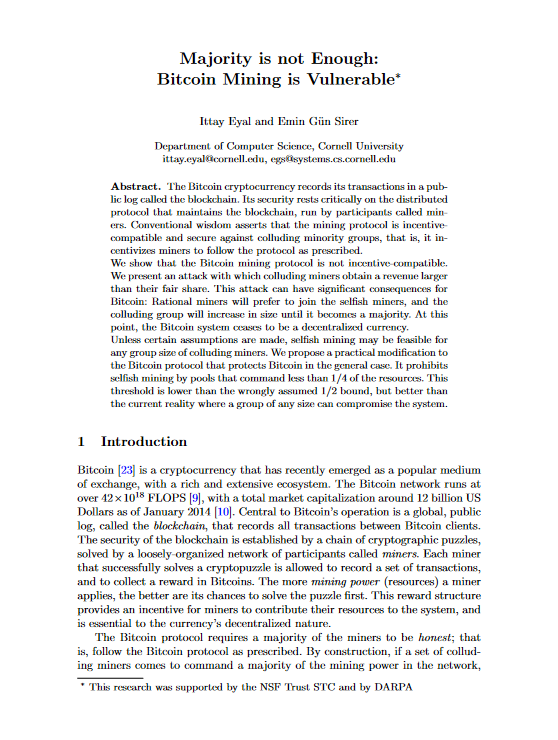
\includegraphics[width = 1.7cm, frame]{../assets/images/Mining_cover}
			\end{column} %\hfill
			\begin{column}{0.8\textwidth}
				\textbf{Majority is not Enough: Bitcoin Mining is Vulnerable} \\ 
				Ittay Eyal and Emin Gün Sirer \\
				\link \href{https://www.cs.cornell.edu/~ie53/publications/btcProcFC.pdf}{Online version}
			\end{column}
		\end{columns}
	%
	

\end{frame}
%%%

\end{document}
